\section{Billedanalyse}

\begin{frame}
\frametitle{Billedanalyse}
\begin{itemize}
\item Kameraet kan give os et billede eller en videosekvens
\item Skal patienten selv tage billeder?
\item Ansigtsgenkendelse hjælper os til at tage et billede af brugeren uden vedkommende ved det

\end{itemize}
\end{frame}


\begin{frame}
\frametitle{Billedanalyse}
\begin{figure}
\centering
\begin{subfigure}[b]{0.45\textwidth}
	\centering
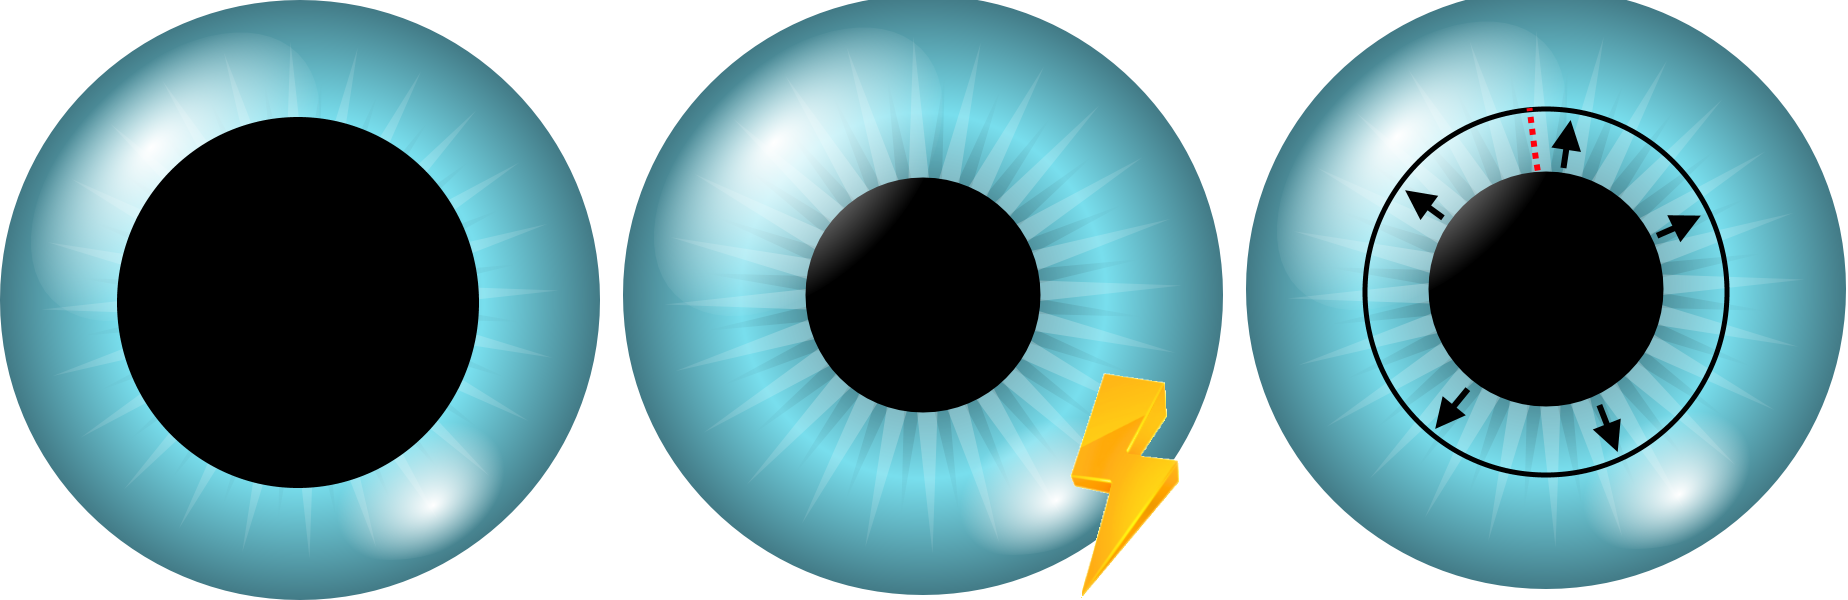
\includegraphics[width=\textwidth]{pupil-dilation}
\caption{Pupil reaktion.}
\end{subfigure}
~~~~
\begin{subfigure}[b]{0.45\textwidth}
	\centering
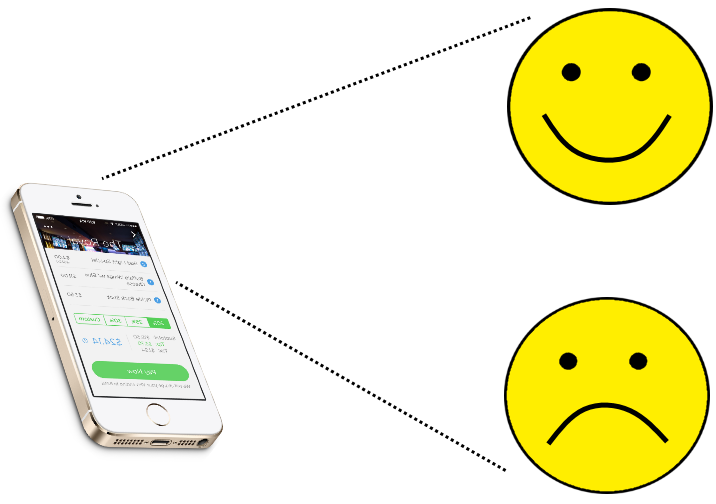
\includegraphics[width=\textwidth]{humoer}
\caption{Humør.}
\end{subfigure}
\caption{Idéer til brug af kameraet.}
\end{figure}

\end{frame}

\section{Accelerometer}
\begin{frame}[fragile]
\frametitle{Accelerometer}
\begin{columns}
\column[t]{5cm}
\begin{itemize}
\item Accelerometeret angiver en retning
\item Gyro sensoren angiver telefonens rotation
\item De kan bruges til evt. at se brugerens gangart
\item Eller til personens aktivitetsniveau
\end{itemize}

\column[t]{5cm}
\begin{figure}

\includegraphics[height=4cm]{red-to-green-gradient-thermometer}
\caption{En måde at visualisere ens aktivitetsniveau.}
\end{figure}
\end{columns}
\end{frame}



\section{Lokation}
\begin{frame}[fragile]
\frametitle{Lokation}
\begin{columns}
\column[t]{5cm}
\begin{itemize}
\item GPS sensoren giver en lokation
\item Kan vise hvor meget brugeren bevæger sig
\item Kan vise steder hvor brugere opholder sig mere end andre
\end{itemize}
\column[t]{5cm}
\begin{figure}
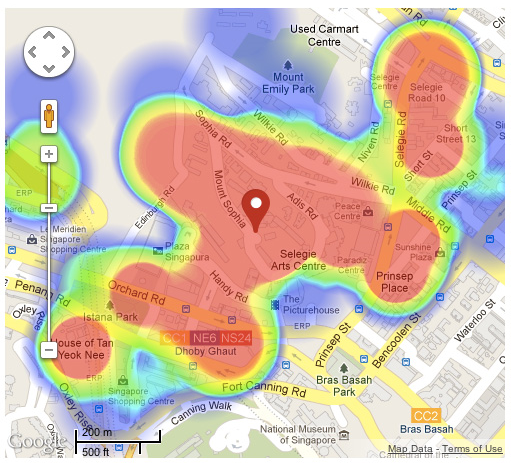
\includegraphics[height=4cm]{heatmap}
\caption{Et heatmap der viser hvor man opholder sig mest.}
\end{figure}
\end{columns}
\end{frame}



\section{Lyd}
\begin{frame}
\frametitle{Lyd}
\end{frame}